% This is samplepaper.tex, a sample chapter demonstrating the
% LLNCS macro package for Springer Computer Science proceedings;
% Version 2.21 of 2022/01/12
%
\documentclass[runningheads]{llncs}
%
\usepackage[T1]{fontenc}
% T1 fonts will be used to generate the final print and online PDFs,
% so please use T1 fonts in your manuscript whenever possible.
% Other font encondings may result in incorrect characters.
%
\usepackage{amsmath}
\usepackage{amssymb}
\usepackage{algorithm}
\usepackage{algorithmic}
\usepackage{graphicx}
%\usepackage{geometry}

\usepackage{tikz}
\usetikzlibrary{arrows.meta, positioning}



% Used for displaying a sample figure. If possible, figure files should
% be included in EPS format.
%
% If you use the hyperref package, please uncomment the following two lines
% to display URLs in blue roman font according to Springer's eBook style:
%\usepackage{color}
%\renewcommand\UrlFont{\color{blue}\rmfamily}
%\urlstyle{rm}
%
\begin{document}
	
	\title{Neuro-Evolved Heuristics for Variable Gapped Common Subsequence Identification}
	%
	\titlerunning{Neural-evolved Heuristics for the VGLCSP}
	
	\author{Marko Djukanović\inst{1, 5}  %\and Nikola Balaban\inst{2}  
		\and
	  Christian Blum\inst{2}  \and 
	  Aleksandar Kartelj\inst{3}  \and
	  Sašo Džeroski\inst{4}  \and
	  Žiga Zebec\inst{5}
	}
	%
	\authorrunning{Djukanovic et al.}
	
	\institute{ University of Nova Gorica, Nova Gorica, Slovenia \\ \email{marko.dukanovic@ung.si} \and 
	%Faculty of Natural Sciences and Mathematics, University of Banja Luka, Banja Luka, Bosnia and Herzegovina
	% \\ 
	%\email{nikola.balaban@student.pmf.unibl.org}, 
%	\email{marko.djukanovic@pmf.unibl.org} \and
		Artificial Intelligence Research Institute (IIIA-CSIC), Barcelona, Spain \\
		\email{christian.blum@iia.csic.es} \and 
		Faculty of Mathematics, University of Belgrade, Belgrade, Serbia \\ \email{kartelj@matf.rs} \\ \and
		Jožef Stefan Institute, Ljubljana, Slovenia \ \\ \email{saso.dzeroski@ijs.si}  \\
		\and
		Institute of Information Sciences (IZUM), Maribor, Slovenia \\
		\email{ziga.zebec@izum.si}
	}
	
	
 
	%
	\maketitle              % typeset  
	
\begin{abstract}
	This study addresses the Variable Gapped Longest Common Subsequence (VGLCS) problem, a variant of the classical longest common subsequence problem that incorporates additional gap constraints. The problem has applications in sequence alignment and time-series analysis. While the two-sequence version has been extensively studied using dynamic programming, its generalized form with multiple input sequences is typically tackled using beam search--based heuristics. However, existing hand-crafted heuristics often suffer from limited robustness.
	
	To overcome this issue, we propose a learning-based approach for automatically designing more effective data-driven heuristics. The heuristics are modeled by a neural network with a predefined architecture, whose weights are optimized by a genetic algorithm in a neuro-evolutionary framework. The learning process alternates between evolutionary optimization of network weights and their evaluation within an iterative multi-source beam search procedure, a state-of-the-art method for the tackled problem. Importantly, the neural network does not directly construct solutions but instead learns to guide the search process, resulting in a neuro-evolved heuristic. 	Furthermore, we introduce an ensemble heuristic that combines the learned heuristics with the best-performing hand-crafted heuristic. The resulting hybrid approach, integrated into the iterative multi-source beam search framework, outperforms existing methods on both synthetic benchmark instances from the literature and the newly introduced real-world instances with data-driven gap constraints.
\end{abstract}

\keywords{Beam search; Neural networks; Neuro-Evolved heuristics; Gap constraints}

\section{Introduction}

The \textit{Longest Common Subsequence Problem} (LCSP)~\cite{DJUKANOVIC2020106499} is a fundamental combinatorial optimization problem with numerous applications in computational biology, particularly in the analysis of molecular sequences. Given a set of input sequences $S=\{s_1,\ldots,s_m\}$ over an alphabet $\Sigma$, the objective is to determine the longest subsequence common to all sequences $s_i \in S$. Over the past decades, several practically motivated variants of LCSP have been proposed by incorporating additional structural or biological constraints, including the constrained, arc-preserving, and repetition-free variants~\cite{lafond2023longest,lin2002longest}.

In this work, we study the \textit{Variable Gapped Longest Common Subsequence Problem} (VGLCSP), introduced in~\cite{penga2011longest}, theoretically analyzed in~\cite{adamson2023longest}, and recently evaluated experimentally in~\cite{djukanovic2026_eurocast}. This variant extends the classical LCSP by introducing flexible gap constraints between consecutive symbols in the subsequence, allowing these gaps to vary along the input sequences.

Formally, for each sequence $s_i \in S$, a gap function $G_{s_i} : \{1,\ldots,|s_i|\} \rightarrow \mathbb{N}$ specifies the maximum allowed distance between consecutive matched positions. If a solution $s$ appears at positions $i_i^1 < \cdots < i_i^{|s|}$ in $s_i$, the gap constraints are satisfied if
\[
i_i^x - i_i^{x-1} \leq G_{s_i}[i_i^x] + 1, \quad \forall x = 2,\ldots,|s|.
\]
A subsequence is feasible if these constraints hold for all sequences $s_i \in S$. The objective is to find the longest feasible subsequence. The VGLCSP provides a flexible and realistic model for sequence alignment, particularly relevant for DNA and protein analysis with variable structural distances, as well as for time-series analysis where events must occur within specified temporal delays~\cite{lainscsek2015delay}.

While several exact dynamic programming approaches exist for the two-sequence case ($m=2$)~\cite{peng2014finding}, the problem becomes computationally intractable for larger $m$; in fact, it is NP-hard in the general case. To date, no efficient exact methods are known for arbitrary $m$. The only available scalable approach is an iterative multi-source beam search (IMSBS)~\cite{djukanovic2026_eurocast}, which explores a state-space representation of the problem. The method iteratively refines candidate root nodes and extends them through feasible symbol additions. Despite its scalability, IMSBS relies on hand-crafted heuristics, which tend to degrade in performance as $m$ increases or the alphabet size $|\Sigma|$ decreases~\cite{DJUKANOVIC2020106499}. The presence of gap constraints further exacerbates this issue.

In addition, existing studies are limited to synthetic benchmark instances, leaving a gap in evaluating methods on realistic data.

To address these limitations, we propose a learning-enhanced beam search framework for VGLCSP. Our approach integrates learned and hand-crafted heuristics into a unified search strategy. The learned heuristic is represented by a multi-layer neural network that scores candidate states during the search. The network parameters are optimized through a genetic algorithm in a neuro-evolutionary framework, where each candidate model is evaluated within the IMSBS procedure. Importantly, the neural model does not directly construct solutions but learns to guide the search process.

Furthermore, we design an ensemble heuristic that combines the learned heuristic with the best-performing hand-crafted heuristic, yielding a more robust guidance mechanism. This hybrid approach is inspired by recent advances in learning-guided combinatorial optimization~\cite{djukanovic2025learning,reixach2024neural,wu2021learning}, but differs in explicitly leveraging complementary heuristic signals within an ensemble.

Finally, to address the lack of realistic benchmarks, we introduce new problem instances derived from biologically motivated datasets, augmented with data-driven gap constraints.

\medskip
\noindent\textbf{Contributions.} The main contributions of this work are:
\begin{itemize}
	\item A neuro-evolutionary framework integrated for learning heuristics in VGLCSP.
	\item An ensemble heuristic combining learned and hand-crafted guidance.
	\item An enhanced IMSBS algorithm integrating the proposed heuristics.
	\item A new set of realistic benchmark instances with data-driven gap constraints.
\end{itemize}
  
The paper is organized as follows. In Section~\ref{sec:imsbs}, the iterative multi source beam search approach from the literature is roughly presented. Section~\ref{sec:ffnn_guidance} provides main details on the process of learning heuristic guidance, and the design of ensemble heuristic estimator for the tacked problem. Section~\ref{sec:experiments} reports a rigorous experimental analysis. Finally, Section~\ref{sec:conclusions} concludes the paper highlighting several future research directions. 
 
 
\section{Iterative Multi-Source Beam Search for the VGLCSP}\label{sec:imsbs}

The first scalable approach for the VGLCSP with an arbitrary number of sequences ($m$) was introduced in~\cite{djukanovic2026_eurocast} as an \textit{Iterative Multi-Source Beam Search} (IMSBS). In this section, we summarize its main components; interested readers are referred to the original paper for full details.

IMSBS is based on a \textit{state graph} representation of the VGLCSP. Each node represents a partial feasible subsequence, characterized by a vector of positions defining a subproblem and the length of the constructed subsequence. Formally, a state $v=(\mathbf{p}^{L,v}, l^v)$ is induced by a partial solution $s^v$ if: (i) $p^{L,v}_i-1$ is the smallest index such that $s^v$ is a subsequence of the prefix $s_i[1]\cdots s_i[p^{L,v}_i-1]$; (ii) $l^v=|s^v|$; and (iii) all gap constraints $G_{s_i}$ are satisfied by $s^v$. 

A directed arc $\alpha=(v_1, v_2)$ labeled by $lett(\alpha)=a \in \Sigma$ exists if $l^{v_2}=l^{v_1}+1$ and $s^{v_2}=s^{v_1}\cdot a$. To expand a state $v$, all letters occurring in the suffixes $S[\mathbf{p}^{L,v}]$ are considered. For each letter $a$, the smallest feasible positions $p^{L,a}_i \geq p^{L,v}_i$ are identified such that the gap constraints are satisfied, i.e., $p^{L,a}_i - p^{L,v}_i \leq G_{s_i}(p^{L,a}_i)$. The resulting child state (if not dominated) is $w=(\mathbf{p}^{L,a}+1, l^v+1)$. Terminal states correspond to non-extendable feasible subsequences.

Unlike the classical LCSP, the VGLCSP admits multiple (potentially exponentially many) root nodes, since starting positions are unconstrained. This may lead to disconnected regions in the state graph. For instance, consider $s_1=\texttt{ATGGAAAA}$ and $s_2=\texttt{ATCCAAAA}$ with $G_{s_1}=G_{s_2}=1$. The root node $((1,1),0)$ cannot reach states with position vector $(5,5)$, thus missing the optimal subsequence $\texttt{AAAA}$. This phenomenon is illustrated in Fig.~\ref{fig:state_graph_vglcs_example}, where the state graph decomposes into disconnected components.

This observation motivates the IMSBS framework, which operates over a dynamically generated set of root nodes explored iteratively. At each iteration, beam search (BS) is applied to selected root nodes. BS is a breadth-first heuristic search strategy~\cite{wiseman2016sequence} that expands a limited number of nodes per level, controlled by the beam width $\beta$, and guided by a heuristic function $h$.

In IMSBS, node selection relies on an upper-bound heuristic defined as
\[
\texttt{UB}(v)= l^v + \sum_{a \in \Sigma} \min_{i=1,\ldots,m} |s_i[p^{L,v}_i, |s_i|]|_a,
\]
which estimates the maximum achievable extension from state $v$. For each letter $a \in \Sigma$, the heuristic evaluates its remaining occurrences in each suffix and aggregates these values to derive an upper bound on the achievable subsequence length.

Despite its scalability, IMSBS relies on hand-crafted heuristics whose effectiveness degrades in challenging settings (e.g., large $m$ or small alphabets), especially under gap constraints. {On top of IMSBS, we develop a learning-based methodology that enhances the search process of the IMSBS through learned heuristic guidance and its integration with existing IMSBS.}
 
\begin{figure}[!ht]
	\centering
	\scalebox{0.6}{
		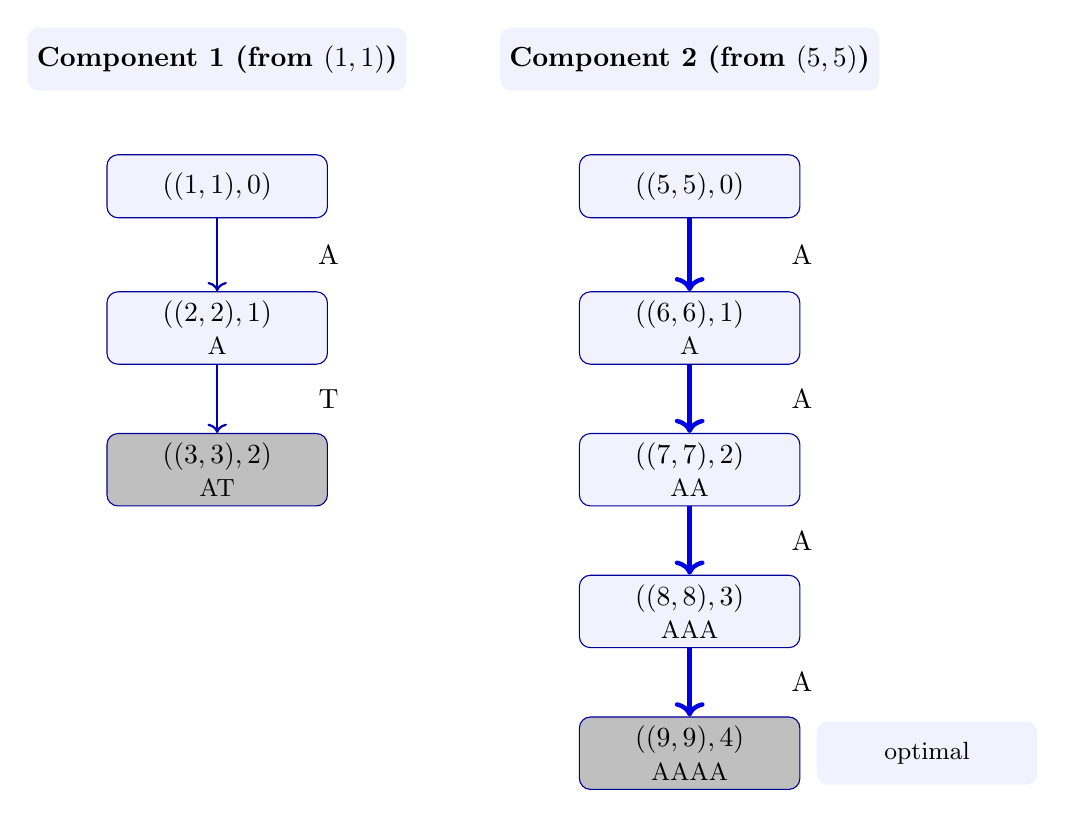
\begin{tikzpicture}[
			node distance=1.8cm,
			every node/.style={
				draw=blue!60!black,
				fill=blue!5,
				rectangle,
				rounded corners,
				minimum width=2.8cm,
				minimum height=0.8cm,
				align=center
			},
			arrow/.style={->, thick, color=blue!70!black},
			optarrow/.style={->, ultra thick, color=blue!90!black}, % highlighted edges
			edgelabel/.style={midway, right, draw=none, fill=none, text=black}
			]
			
			% -------- Component 1 --------
			\node (r1) at (0,0) {$((1,1),0)$};
			\node (a1) [below of=r1] {$((2,2),1)$\\\small A};
			\node[fill=lightgray] (t1) [below of=a1] {$((3,3),2)$\\\small AT};
			
			\draw[arrow] (r1) -- node[edgelabel] {A} (a1);
			\draw[arrow] (a1) -- node[edgelabel] {T} (t1);
			
			% -------- Component 2 --------
			\node (r2) at (6,0) {$((5,5),0)$};
			\node (a2) [below of=r2] {$((6,6),1)$\\\small A};
			\node (a3) [below of=a2] {$((7,7),2)$\\\small AA};
			\node (a4) [below of=a3] {$((8,8),3)$\\\small AAA};
			\node[fill=lightgray] (a5) [below of=a4] {$((9,9),4)$\\\small AAAA};
			
			\draw[optarrow] (r2) -- node[edgelabel] {A} (a2);
			\draw[optarrow] (a2) -- node[edgelabel] {A} (a3);
			\draw[optarrow] (a3) -- node[edgelabel] {A} (a4);
			\draw[optarrow] (a4) -- node[edgelabel] {A} (a5);
			
			\node[draw=none, right=0.2cm of a5] {\small optimal};
			
			% -------- Titles --------
			\node[draw=none, above=0.8cm of r1] {\textbf{Component 1 (from $(1,1)$)}};
			\node[draw=none, above=0.8cm of r2] {\textbf{Component 2 (from $(5,5)$)}};
			
	\end{tikzpicture}}
	\caption{State graph for $s_1=\texttt{ATGGAAAA}$ and $s_2=\texttt{ATCCAAAA}$ with $G_{s_1}=G_{s_2}=1$. The state graph consists of two disconnected components. Starting from $(1,1)$ leads to a suboptimal solution, while starting from $(5,5)$ yields the optimal subsequence $\texttt{AAAA}$.}
	\label{fig:state_graph_vglcs_example}
\end{figure}
	 
	 
	% In the IMSBS, BS is iteratively executed on a set of promising candidate root nodes as an initial beam, selected from a dynamically maintained global priority queue of candidate root nodes, controlling the diversification of the approach.	
	 
	 %Each iteration performs a complete BS on a few  ($num\_root\_nodes$) top candidate root nodes, which are, beforehand, refined by the beam search with a small beam width $\beta'$ and heuristic guidance $h'$, as not all candidate nodes will represent real root nodes. This process intensifies the search and permits it from returning proven suboptimal solutions. During each BS call, new candidate root nodes are generated from the complete (non-expandable) nodes and have been subsequently added to the priority queue. This approach provides a balance the intensification and diversification by involving several parameters. The stopping criteria utilized for the IMSBS are the number of allowed beam search iterations ($bs\_iters$), and the time limit of 30 minutes per each run.
	
	In the subsequent part of the paper, we refer to the algorithm as \texttt{IMSBS},  %($\beta, h, \beta'$, $h', num\_root\_nodes$), 
	returning an approximate solution $s_{imsbs}$.  %with three additional strategic parameters following~\cite{djukanovic2026_eurocast}.  
 
   
\section{Learning to Guide the Search} \label{sec:ffnn_guidance}

Neural networks (NNs) are well-established machine learning models~\cite{gurney2018introduction,bishop1994neural} that have demonstrated strong performance across a wide range of domains. They range from simple multi-layer perceptrons (MLPs) to more complex convolutional and recurrent architectures~\cite{mienye2024recurrent}. In this work, we focus on fully connected multi-layer perceptrons to design an alternative, data-driven heuristic for guiding the IMSBS procedure~\cite{djukanovic2026_eurocast}. 

The key challenge lies in parameterizing the neural model such that it provides meaningful guidance during the search. Specifically, the network is trained to assign a score to each node (i.e., subproblem), based on features extracted from the corresponding partial solution and its associated residual problem.

In standard neural network training, parameters are optimized via forward and backward propagation, typically using gradient-based methods such as (stochastic) gradient descent~\cite{amari1993backpropagation}. However, in our setting—characterized by a combinatorial \textsc{NP}-hard problem—target values are not readily available, especially for large instances. This limits the applicability of supervised learning approaches. Instead, we adopt a population-based metaheuristic approach, where candidate NN configurations are evaluated indirectly through their impact on the performance of the IMSBS algorithm. 

\medskip
\noindent\textbf{Predefined NN Architecture.}
The heuristic is modeled as a multi-layer perceptron consisting of an input layer, several hidden layers with user-defined sizes, and a single output neuron. The input layer receives a vector of numerical features describing the current search state, while the output represents the estimated promise of expanding that state.

For each layer $l$, forward propagation is defined as
\[
\mathbf{z}^{(l+1)} = W^{(l)} \mathbf{a}^{(l)} + b^{(l)}, \quad
\mathbf{a}^{(l+1)} = \phi(\mathbf{z}^{(l+1)}),
\]
where $W^{(l)}$ and $b^{(l)}$ denote the weights and biases, and $\phi$ is a non-linear activation function (e.g., \texttt{tanh}, \texttt{ReLU}, or \texttt{sigmoid}). The final pre-activation value is used as the heuristic score. All parameters are flattened into a single vector $w=\texttt{flatten}(W,b)$, which represents an individual in the evolutionary process.

\medskip
\noindent\textbf{Fitness Evaluation.}
Given a candidate weight vector $w$, the evaluation proceeds as follows: 
(i) the weights are loaded into the NN architecture $\mathcal{N}$; 
(ii) IMSBS is executed on each instance from a training set $\mathcal{T}$ using the neural heuristic $h_w$; and 
(iii) the best solution quality obtained per instance is recorded. 
The fitness of $w$ is defined as the average solution quality over $\mathcal{T}$:
\begin{equation} \label{eq:training_problem_optimization}
	\max_{w} \; \emph{Fitness}(w)=\frac{1}{|\mathcal T|} \sum_{I \in \mathcal{T}} f(\texttt{IMSBS}(I, h_w)),
\end{equation}
where $f(\cdot)$ denotes the length of the best subsequence found. Validation performance is computed analogously on a separate dataset $\mathcal{V}$.

\medskip
\noindent\textbf{Feature Extraction.}
To guide the search effectively, each node $v=(\mathbf{p}^v, l^v)$ is mapped to a fixed-length feature vector capturing both the construction progress and the structure of the induced subproblem. The design is instance-independent and robust across varying problem sizes.

Let $S=\{s_1,\ldots,s_m\}$ denote the input sequences. The position vector $\mathbf{p}^v$ is first normalized by sequence lengths:
\[
F^v_i = \frac{p^v_i}{|s_i|}, \quad i=1,\ldots,m,
\]
ensuring scale invariance. From this normalized vector, we extract four statistics: $\max(\mathbf{F}^v)$, $\min(\mathbf{F}^v)$, $\texttt{mean}(\mathbf{F}^v)$, and $\texttt{std}(\mathbf{F}^v)$, capturing the progress and imbalance across sequences. The current subsequence length $l^v$ is also included.

To reflect future feasibility, we compute gap-related statistics:
\[
G^{\min}, \; G^{\max}, \; G^{\texttt{avg}}, \; G^{\texttt{std}},
\]
evaluated over the remaining positions in all sequences. These features quantify the flexibility of future extensions: larger gaps indicate more freedom, while smaller or highly variable gaps suggest tighter constraints.

Finally, two global features—alphabet size $|\Sigma|$ and the number of sequences $m$—are included. All features are standardized to zero mean and unit variance prior to training. The resulting 11-dimensional representation provides a compact yet expressive description of each search state.

\medskip
\noindent\textbf{Optimization of NN Parameters.}
To optimize the NN parameters, we employ a \textit{Biased Random-Key Genetic Algorithm} (BRKGA), a population-based evolutionary method. Each individual encodes a candidate weight vector $w$, initialized uniformly at random in the interval $[-q,q]$ with $q=1$. The evolutionary process iteratively refines the population toward high-quality heuristics $h_w=\mathcal{N}(w)$, where $\mathcal{N}$ is a predefined NN architecture, based on the fitness defined in Eq.~(\ref{eq:training_problem_optimization}). The overall learning mechanism is summarized in Algorithm~\ref{alg:learning_mechanism}.


\begin{algorithm}[!ht]
	\caption{GA-Based Learning of a Beam Search Heuristic} \label{alg:learning_mechanism}
	\begin{algorithmic}[1]
		\STATE \textbf{Input}: NN architecture $\mathcal{N}$, IMSBS parameters, BRKGA parameters, training set $\mathcal{T}$, validation set $\mathcal{V}$
		\STATE \textbf{Output}: optimized weight vector $w^\ast$
		\STATE Initialize population $P$ with random weight vectors
		\STATE Evaluate all individuals on $\mathcal{T}$
		\STATE $w^\ast \leftarrow$ best individual in $P$
		\WHILE{time limit $t_{\max}$ not exceeded}
		\STATE Sort $P$ in descending order of \emph{Fitness}
		\STATE Initialize new population $P'$
		\STATE Copy top $n_{\text{elite}}$ individuals from $P$ to $P'$
		
		\FOR{$i = 1$ to $n_{\text{mutants}}$}
		\STATE Generate random individual $x$
		\STATE Evaluate $x$ on $\mathcal{T}$ and add to $P'$
		\STATE Update $w^\ast$ if improved and validation does not degrade
		\ENDFOR
		
		\FOR{$i = 1$ to $n_{\text{offspring}}$}
		\STATE Select one elite parent and one non-elite parent
		\STATE Generate offspring via biased crossover ($p_{\text{bias}}$)
		\STATE Evaluate offspring on $\mathcal{T}$ and add to $P'$
		\STATE Update $w^\ast$ if improved and validation does not degrade
		\ENDFOR
		
		\STATE $P \leftarrow P'$
		\ENDWHILE
		\STATE \textbf{return} $w^\ast$
	\end{algorithmic}
\end{algorithm}


 
 
 \textbf{Overall Learning Procedure.}
 The proposed learning framework alternates between evolutionary optimization of neural network parameters and their evaluation within the IMSBS procedure. Importantly, the neural network does not directly construct solutions; instead, it learns to \emph{guide} the search process. This places the approach within the class of neuro-evolutionary hyper-heuristics.
 
 Given a predefined NN architecture $\mathcal{N}$, IMSBS parameters, and BRKGA parameters, the procedure begins by generating an initial population $P$ of candidate weight vectors. Each individual is evaluated on the training set $\mathcal{T}$ using IMSBS guided by the corresponding neural heuristic. The best-performing solution is stored as $w^\ast$. In our implementation, IMSBS is executed with parameters $\beta=500$ and $\texttt{beam\_iters}=100$, while the remaining parameters follow~\cite{djukanovic2026_eurocast}. This configuration provides a suitable balance between computational cost and robustness during training.
 
 The evolutionary process proceeds iteratively as follows. The population is first sorted according to fitness. A new population $P'$ is then constructed by preserving the top $n_{\text{elite}}$ individuals (elitism), introducing $n_{\text{mutants}}$ randomly generated individuals (diversification), and generating $n_{\text{offspring}}$ offspring via biased crossover. In each crossover, one parent is selected from the elite set and the other from the remaining population. Each gene (weight) is inherited from the elite parent with probability $p_{\text{bias}} \geq 0.5$, and from the second parent otherwise.
 
 Each newly generated individual is evaluated on $\mathcal{T}$. Whenever an improved solution is found, its performance is additionally assessed on the validation set $\mathcal{V}$. To mitigate overfitting, we adopt an early stopping strategy: if the validation performance deteriorates, the update is discarded.
 
 The process repeats until a time limit $t_{\max}$ is reached (set to 2 CPU hours). The algorithm returns the best weight vector $w^\ast$, corresponding to the neural network $\mathcal{N}(w^\ast)$ that induces the most effective heuristic $h_w$.
 
 In our experiments, the BRKGA parameters are set to $n_{\text{pop}}=20$, $n_{\text{elite}}=1$, $p_{\text{bias}}=0.5$, and $n_{\text{mutants}}=7$. A visualization of the learning process is provided in Fig.~\ref{fig:ga_imsbs}.

\begin{figure}[!ht]
	\centering
	\scalebox{0.55}{
		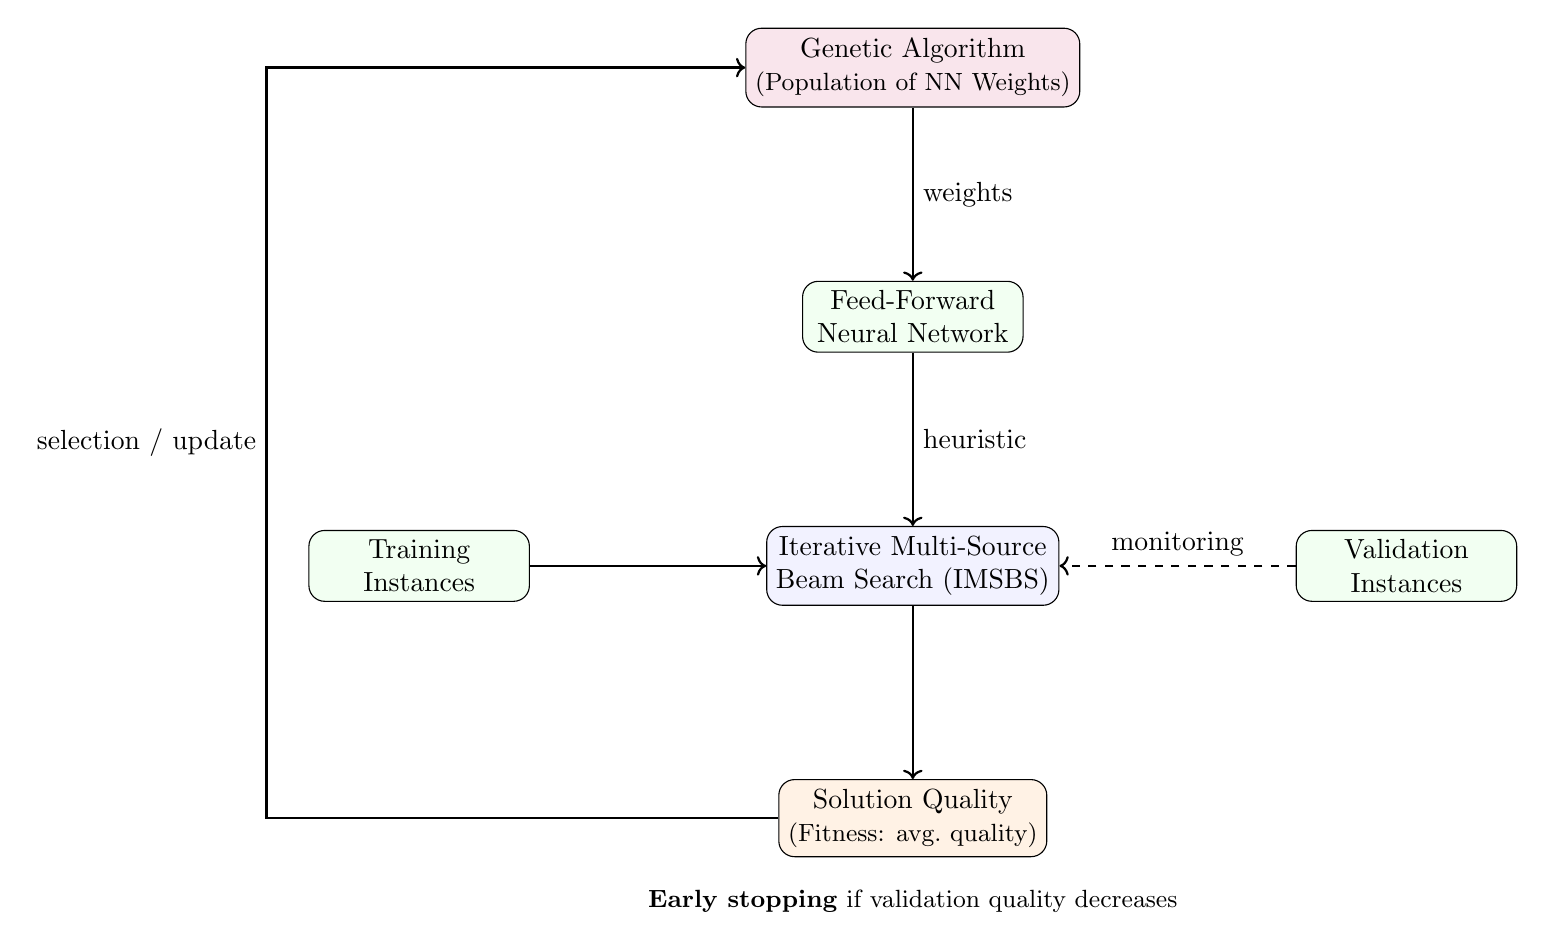
\begin{tikzpicture}[
			box/.style={draw, rounded corners=2mm, align=center, minimum width=3.4cm, minimum height=1cm, fill=blue!5},
			smallbox/.style={draw, rounded corners=2mm, align=center, minimum width=2.8cm, minimum height=0.9cm, fill=green!5},
			evalbox/.style={draw, rounded corners=2mm, align=center, minimum width=3cm, minimum height=0.9cm, fill=orange!10},
			arrow/.style={->, thick},
			dashedarrow/.style={->, thick, dashed},
			node distance=2.2cm
			]
			
			% --- GA ---
			\node[box, fill=purple!10] (ga) {Genetic Algorithm\\\small (Population of NN Weights)};
			
			% --- NN ---
			\node[smallbox, below=of ga] (nn) {Feed-Forward\\Neural Network};
			
			% --- Beam Search ---
			\node[box, below=of nn] (bs) {Iterative Multi-Source\\Beam Search (IMSBS)};
			
			% --- Training ---
			\node[smallbox, left=3cm of bs] (train) {Training\\Instances};
			
			% --- Validation ---
			\node[smallbox, right=3cm of bs] (val) {Validation\\Instances};
			
			% --- Fitness ---
			\node[evalbox, below=of bs] (fitness) {Solution Quality\\\small (Fitness: avg.\ quality)};
			
			% --- Arrows ---
			\draw[arrow] (ga) -- node[right]{weights} (nn);
			\draw[arrow] (nn) -- node[right]{heuristic} (bs);
			
			\draw[arrow] (train) -- (bs);
			\draw[dashedarrow] (val) -- node[above]{monitoring} (bs);
			
			\draw[arrow] (bs) -- (fitness);
			
			% --- Rectangular loop around training node ---
			\draw[arrow] (fitness.west) -- ++(-6.5,0)          % go left past training node
			|- node[pos=0.25,left]{selection / update} (ga.west);
			
			% --- Optional annotation ---
			\node[below=0.3cm of fitness] {\small \textbf{Early stopping} if validation quality decreases};
			
	\end{tikzpicture}}
	
	\caption{Enhanced learning framework integrating a Genetic Algorithm with IMSBS.
		The GA evolves neural network weights, which define a heuristic used within the beam search.
		Training instances guide optimization, while validation instances monitor generalization.
		The feedback loop updates the population based on solution quality.}
	\label{fig:ga_imsbs}
\end{figure}
 
    
  \subsection{An ensemble approach}
    
    According to the preliminary results, the learning heuristics performs in overall better than the competitor hand-crafted heuristic from the literature. However, not for all cases, and especially on the instances with small $m$.  In order to improve the results further, we employ a rank-based ensemble strategy that combines a learned heuristic with an analytical hand-crafted upper bound ($\text{UB}$)~\cite{djukanovic2026_eurocast}, see Section~\ref{sec:imsbs}.  Specifically, each candidate node in beam search is evaluated using two criteria: a neural score obtained from a FFNN $\mathcal{N}(w^*)$, denoted $h_{w^*}=\mathcal{N}({w^*})$,  and  a problem-specific hand-crafted $\text{UB}$. 
    
    Instead of combining the raw scores directly, which may differ in scale and distribution, we adopt a rank aggregation approach. First, candidate nodes are sorted independently according to each criterion, producing two rankings. Each node is then assigned a rank based on its position in each sorted list.   The final ranking score is computed as a weighted combination of the two ranks:
    \begin{equation}\label{eq:ensemble_heuristic}
        r(v) = \alpha \cdot r_{h_{w^*}}(v) + (1 - \alpha) \cdot r_{\text{UB}}(v),
    \end{equation}
    %where $\alpha = 0.45$ is set in our implementation except for $m=3$ where $\alpha=0.5$ is used. 
    Nodes are then sorted in ascending order of $r(v)$, and the top candidates are retained according to the beam width. This rank-based ensemble heuristic provides a robust mechanism for integrating learned and analytical guidance, mitigating scale inconsistencies and improving search stability. 
     
% The proposed framework learns heuristics rather than explicit solutions. The neural network is optimized exclusively through downstream search performance, enabling learning in non-differentiable settings. This tightly coupled integration of evolutionary learning and the classical optimization algorithm Beam Search allows the system to adapt its guidance strategy to the structure of the problem instances.
 
 \section{Experimental Evaluation}\label{sec:experiments}
   
In this section we compare the performance of the two methods: (i) \textsc{Imsbs}: a baseline state-of-the-art iterative beam search strategy from~\cite{djukanovic2026_eurocast}, and  (ii) \textsc{Limsbs}-ensamble: a \textsc{Imsbs} guided by ~(\ref{eq:ensemble_heuristic}).  All approaches are implemented in C++ and compiled via GCC compiler,  evaluated on the VEGA HPC system, hosted at IZUM, Maribor, Slovenia. The cluster consists of 960 compute nodes equipped with the AMD EPYC 7H12 CPUs operating at 2.35\,GHz. All experiments were conducted in a single-threaded setting.  

\textbf{Benchmark instances}. For the evaluation purposes, two type of benchmark sets are used. The first set of synthetic instances is proposed in~\cite{djukanovic2026_eurocast}. For each combination of  $n \in \{50, 100, 200, 500\}$, $m \in \{2, 3, 5, 10\}$, and $|\Sigma| \in \{2, 4\}$, 10 random problem instances are randomly generated, a total of   \textit{320 problem instances}. The benchmark set is denoted as \textsc{Random}. Apart from these, a set of biologically-motivated VGLCSP instances are introduced here.  

In the context of real instances,  we will be modeling context-dependent importance of positions of sequences that represents gap values.  It aligns with  sequence alignment scoring and %, attention mechanisms, and  
 weighted subsequence problems. Interpretation of these context relies on the fact that higher weights on positions refer to  stronger influence of these nucleotides in forming reliable connections with other (neighboring) acids in common subsequences. 
Stability ranking between pairs of nucleotides is (statistically) determined in the fundamental works on electrostatic interactions and structural influence~\cite{santalucia1998unified,watkins2005nearest}, used here in creating energy-aware LCS solutions, i.e., structure-aware variable-gap sequences (data-driven constraints):
%\textit{Energy-aware LCS / weighted subsequence}.

$\texttt{DINUC\_WEIGHT} = \{
`\text{AA}':1.00, `\text{TT}':1.00,
`\text{AT}':0.88, `\text{TA}':0.58,
`\text{CA}':1.45, `\text{TG}':1.45,
`\text{GT}':1.44, `\text{AC}':1.44,
`\text{CT}':1.28, `\text{AG}':1.28,
`\text{GA}':1.30, `\text{TC}':1.30,
`\text{CG}':2.17,
`\text{GC}':2.24,
`\text{GG}':1.84, `\text{CC}':1.84
\}$
'\text{AA}' and its score 1.00 means 
the stability of interactions between nucleotides $\texttt{A}$ and $\texttt{A}$ assign a value of 1.0. 
%
  In essence,  {value of gap constraint at each position will be proportional to local thermodynamic stability estimated via nearest-neighbor interactions around the nucleotide placed at that position.} \textit{Dinucleotide-based structural model} is defined as a dinucleotide weight function: $
f(s[i], s[i+1]) = -\Delta G(s[i], s[i+1]),
$
where $\Delta G$ denotes the nearest-neighbor free energy estimated by \texttt{DINUC\_WEIGHT}. 

To ensure consistency with the directional nature of the gapped LCS constraint, a \emph{causal} positional contribution is derived. Each position $k$ of a sequence $s$ is associated only with the interaction formed with its immediate predecessor:

$
f^s_k =
\begin{cases}
	f(s[{k-1}], s[k]), & k > 1, \ \\
	0, & k = 1.
\end{cases}
$

 Each position inherits structural influence from the bond linking it to the previous nucleotide. First position has no predecessor and is therefore assigned zero contribution.
  This definition enforces a left-to-right dependency structure, ensuring that all subsequent computations of influence and gap constraints depend only on previously observed positions. This is consistent with the feasibility condition in the gapped LCS problem, where admissibility of extending a subsequence depends on the last selected position.

%In order to align the influence model with the semantics of the gapped LCS constraint, we define influence in a \emph{causal} (left-to-right) manner.

The influence at position $i$ is computed using only preceding positions:
$
I^{s}(i) = \sum_{k=\max(1,i-r)}^{i} e^{-\lambda (i-k)} \cdot f^{s}_k$.  This formulation reflects the fact that, in the gapped LCS problem, feasibility of selecting position $i$ depends on the previously selected position. %Therefore, the structural context relevant to $i$ must be derived exclusively from preceding positions. 
Note that $r$ is a parameter.  The resulting influence values induce \emph{directional structure} in the sequence: (i) regions preceded by strong interactions accumulate high influence, (ii) regions following weak or irregular segments exhibit lower influence.

In order to normalize these values,  we employ the following formula:

$$
\hat{I}^{(j)}_i = \frac{I^{(j)}_i - \min(I^{(j)})}{\max(I^{(j)}) - \min(I^{(j)}) + \epsilon} \in \left[0, 1 \right],
$$

and gap constraints are obtained via a \emph{direct mapping}:  $
w^{(j)}_i = w_{\min} + (w_{\max} - w_{\min}) \cdot \hat{I}^{(j)}_i.
$
 In this context,  high influence refers to large allowed gap, whilst low influence refers to restrictive gap.

This mapping reflects the idea that positions with strong structural connectivity can support longer-range dependencies allowing more flexible matching. Interval $[w_{\min}, w_{\max}]$ is parametrized, here  fixed to 1 and 10, respectively.  



The described  instance generator is based on the following parameters: $r$ as influence radius, $\lambda$ as decay factor, $[w_{\min}, w_{\max}]$ as gap bounds. We additionally fixed $r=10$, and $\lambda=0.5$. 
% By linking gap constraints directly to structural influence, the generator produces instances with controllable heterogeneity and realistic dependency patterns. 
The resulting benchmark enable systematic evaluation of multi-sequence gapped LCS algorithms under diverse and challenging conditions.
 
 To demonstrate effectiveness of the designed approaches on real-world instances, we have used well-known LCS benchmark sets \textsc{Rat} and \textsc{Virus}~\cite{DJUKANOVIC2020106499}. For each input sequence in each problem instance, we have induced a respective data-driven gap constraint by the above  methodology.
  We consider only the instances with $|\Sigma|=4$ in both datasets, as the gap involvement for the instance with  $|\Sigma|=20$ induced a rather short solutions found by the approaches---therefore hardly relevant from the biological standpoint.  
 The generated dataset, denoted by \textsc{Real},  comprises $2\cdot 10=20$ problem instances. All sequences have a length of 600, and, as already mentioned, differentiate by $m$, ranging from 10 to 200. 


%\textit{Noise Injection}. 

%$
%w^{(j)}_i \leftarrow w^{(j)}_i + \mathcal{N}(0, \sigma^2),
%$
%followed by clipping to $[w_{\min}, w_{\max}]$.

 All benchmark sets are freely available at   
\url{XX}. \textcolor{red}{TODO: Revise } \\
 
\textbf{Tuning process.}   \textsc{Imsbs} parameters are tuned on benchmark set \textsc{Random}  by employing \texttt{irace}~\cite{perez2014analysis},  with an allowed training budget of 5000 runs (each run is limited to an execution time of 30 minutes) producing the following \textsc{Imsbs} configuration:   $\beta=3000$, $h=\text{UB}$, and   $\#imbs\_iters=5000$. One instance from each group has been used for the training, thus 32 problem instances in overall. 
 
 All other (less sensible) parameters are set to the values reported in~\cite{djukanovic2026_eurocast}.  Concerning the learning  \textsc{Limsbs}-ensemble approach, it inherits the same setting form \textsc{Imsbs}, to be completely fair with the comparison. For the learning process, we experimented with different architectures for NN:  2-layer structures with 5 and 10 neurons per layer, and 3-layer configurations    with  5 and 10 neurons. 
 
In order to reduce time for tuning different neural network architecture, we allow setting up the same activation function at each layer, selecting among three (most) known: $\{\texttt{tanh}, \texttt{ReLU}, \texttt{sigmoid}\}$. To measure the sensibility analysis w.r.t. set of (11) involved features, we have split them into three groups: (i) {Feature configuration 1} $F_1$ involves 4 features extracted from input sequences, 4 features extracted from gap constraints, and length of partial solution; (ii) When adding  $|\Sigma|$ to $F_1$, we get feature configuration $F_2$; (iii) When adding  $m$  to $F_2,$ we obtain the feature configuration $F_3$. 

After exhaustive training evaluations, we opt to chose the following configurations for the architecture of neural networks, one per different $m$ in the case of benchmark set \textsc{Random}:
\begin{itemize}
	\item $m=2$: units at each layer of FFNN is (10, 5, 5); activation function is \texttt{ReLu}; and the feature set $F_2$;
	\item $m=3$: units at each layer of FFNN set to (10, 10, 5); activation function is set to  \texttt{ReLu}; and the feature set to $F_2$;
	\item $m=5$: units at each layer of FFNN set to (10, 5, 5), activation function set to \texttt{sigmoid}, and the feature set to $F_1$;
	\item $m=10$: units at each layer of FFNN set to (10, 5, 5);   activation function set to \texttt{ReLu}, and the feature set to $F_2$. 
\end{itemize}
The parameter  $\alpha = 0.45$ in our ensemble approach except for $m=3$ where $\alpha=0.5$ as the results of grid search.   We employed 32 instances for the training instances $\mathcal{T}$ and the same amount for the validation instances $\mathcal{V}$; one instance is selected randomly per each (32) group from benchmark set \textsc{Random}. Thus, eight instances are used per each learning process---split by different $m$---for training and validation purposes.


For the benchmark set \textsc{Real}, the employed architecture of NN is the same utilized for the benchmark set \textsc{Random} and the  largest $m=10$ case. This is because we wanted to test the robustness of the learned heuristic on  other than random instance distributions with a large number of sequences ($m$). Note that  all 20 instances have 10 or more sequences. The parameters of \textsc{Imsbs} follows those settings from the benchmark set \textsc{Random}.  \\

\subsection{Numerical results on  benchmark set \textsc{Random}}

  
\begin{table}[t]
	\centering
	\caption{Comparison of objective values between \textsc{Imsbs} and \textsc{Limsbs}-ensemble on benchmark set \textsc{Random}. Best results per instance category are displayed in bold.}
	\label{tab:preliminary_results}
	
	\begin{minipage}{0.4\textwidth}
		\centering
		\setlength{\tabcolsep}{4pt}
		\renewcommand{\arraystretch}{1.1}
		\scalebox{0.8}{
			\begin{tabular}{cll|ll}
				\hline
				$m$ & $n$ & $|\Sigma|$ & \textsc{Limsbs}-ensemble & \textsc{Imsbs} \\ \hline
2 &  50 & 2 & 37.3 & \textbf{37.7} \\
2 &  50 & 4 & \textbf{30.1} & \textbf{30.1} \\
 2 & 100 & 2 & 72.4 & \textbf{72.9} \\
2 & 100 & 4 & \textbf{62.0} & 61.9 \\
2 & 200 & 2 & \textbf{142.5} & 139.3 \\
2 & 200 & 4 & \textbf{125.9} & 125.5 \\
2 & 500 & 2 & \textbf{305.9} & 282.1 \\
2 & 500 & 4 & \textbf{305.5} & 303.0 \\ \hline
3 &  50 & 2 & \textbf{31.2} & \textbf{31.2} \\
3 &  50 & 4 & \textbf{22.9} & \textbf{22.9} \\
3 & 100 & 2 & \textbf{58.5} & \textbf{58.5} \\
3 & 100 & 4 & \textbf{48.7} & 48.5 \\
3 & 200 & 2 & \textbf{106.7} & 106.4 \\
3 & 200 & 4 & \textbf{97.9} & 97.8 \\
3 & 500 & 2 & \textbf{154.9} & 150.6 \\
3 & 500 & 4 & \textbf{237.6} & 236.0 \\
				\hline \hline
Avg. &  &  & \textbf{115.0}  & {112.8} \\ \hline \hline
		\end{tabular}}
	\end{minipage}
	\hfill
	\begin{minipage}{0.4\textwidth}
		\centering
		\setlength{\tabcolsep}{4pt}
		\renewcommand{\arraystretch}{1.1}
		\scalebox{0.8}{
			\begin{tabular}{cll|ll}
				\hline
				$m$ & $n$ & $|\Sigma|$ & \textsc{Limsbs}-ensemble & \textsc{Imsbs} \\
				\hline
 5 &  50 & 2 & \textbf{20.5} & \textbf{20.5} \\
5 &  50 & 4 & \textbf{15.3} & \textbf{15.3} \\
 5 & 100 & 2 & 32.6 & \textbf{32.9} \\
 5 & 100 & 4 & 28.0 & \textbf{28.1} \\
 5 & 200 & 2 & \textbf{45.5} & 42.1 \\
 5 & 200 & 4 & \textbf{41.8} & 38.8 \\
 5 & 500 & 2 & \textbf{45.7} & 39.2 \\
 5 & 500 & 4 & \textbf{58.0} & 45.6 \\ \hline
 10 &  50 & 2 & \textbf{11.7} & \textbf{11.7} \\
 10 &  50 & 4 & 7.3 & \textbf{7.5} \\
 10 & 100 & 2 & \textbf{14.3} & 12.0 \\
 10 & 100 & 4 & \textbf{9.6} & 8.9 \\
 10 & 200 & 2 & \textbf{14.3} & 12.8 \\
 10 & 200 & 4 & \textbf{9.4} & 8.2 \\
 10 & 500 & 2 & \textbf{14.3} & 13.2 \\
 10 & 500 & 4 & \textbf{10.0} & 8.6 \\
				\hline \hline
Avg. &    &   &   \textbf{23.6}    & 21.6 \\ \hline \hline
		\end{tabular}}
	\end{minipage}
	\vspace{-0.5cm}
\end{table}
  
These results are presented in Table~\ref{tab:preliminary_results} which consists of two blocks: the first gives an instance group description, the  next block is reserved for the results of \textsc{Limsbs}-ensemble and \textsc{Imsbs} approaches, reporting the average results of each group (over 10 instances). 
  
  
 Additionally, we evaluated the difference in solution quality between \textsc{Limsbs}-ensemble and \textsc{Imsbs} using the Wilcoxon signed-rank test on paired instances, reported in Table~\ref{tab:statistical_test}. 
 
 
 \begin{table}[!ht]
 	\centering
 	\caption{Statistical comparison between \textsc{Limsbs}-ensemble and \textsc{Imsbs} using the Wilcoxon signed-rank test (one-sided).}
 	\label{tab:statistical_test}
 	\scalebox{0.85}{
 	\begin{tabular}{lccc}
 		\hline
 		\textbf{Comparison} & \textbf{Wins / Ties / Losses} & \textbf{p-value} & \textbf{Conclusion} \\
 		\hline
 		All instances ($m = 2,3,5,10$) & 20 / 7 / 5 & 0.009 & LIMSBS significantly better \\
 		Small instances ($m = 2,3$)    & 10 / 4 / 2  & $<0.01$ & Significant difference \\
 		Large instances ($m = 5,10$)   & 10 / 3 / 3 & $< 0.05$ & LIMSBS significantly better \\
 		\hline
 	\end{tabular}}
    \vspace{-0.5cm}
 \end{table}

The test reveals a statistically significant difference in favor of \textsc{Limsbs}-ensemble, indicating that the learned approach achieves superior performance overall. Out of 32 instances, \textsc{Limsbs}-ensemble outperforms \textsc{Imsbs} in 20 cases, while 7 instances result in ties and only 5 favor \textsc{Imsbs}. 

\subsection{Numerical results on benchmark set \textsc{Real}}
   The results are reported in
Table~\ref{tab:real_results}, organized in a similar manner as Table~\ref{tab:preliminary_results} (with additional columns, reporting the runtimes of each approach per instance ($t[s]$) and lengths of the best LCS from the literature~\cite{DJUKANOVIC2020106499} (LCS$^*$)).  The following conclusions are drawn. 

 \begin{table}[!ht]
	\centering
	\caption{Comparison of \textsc{Limsbs}-ensemble and \textsc{Imsbs} on benchmark set \textsc{Real}.}
	\label{tab:real_results}
	
	\begin{minipage}{0.45\textwidth}
		\centering
		\textbf{RAT instances}
		\begin{tabular}{l|lr|lr}
			\hline
			$m$ & \textsc{Limsbs}-ensemble & $\overline{t}[s]$ & \textsc{Imsbs} & $\overline{t}[s]$ \\
			\hline \hline
			10 & \textbf{28} & 43.44 & 25          & 30.65 \\
			15 & \textbf{11} & 23.39 & \textbf{11} & 24.26 \\
			20 & \textbf{10} & 11.31 & 9           & 49.36 \\
			25 & \textbf{9}  & 17.53 & 7           & 29.62 \\
			40 & \textbf{5}  & 18.18 & 4           & 48.64 \\
			60 & \textbf{3}  & 22.62 & 1           & 45.22 \\
			80 & \textbf{1}  & 22.52 & \textbf{1}  & 53.02 \\
			
			100 & \textbf{1}  & 25.71 & \textbf{1}  & 44.30 \\

			150 & \textbf{1}  & 39.51 & \textbf{1}  & 66.57 \\

			200 & \textbf{1}  & 39.82 & \textbf{1}  & 62.54 \\

			\hline
		\end{tabular}
	\end{minipage}
	\hfill \hfill
	\begin{minipage}{0.45\textwidth}
		\centering
		\textbf{VIRUS instances}
		\begin{tabular}{l|lr|lr}
			\hline
			$m$ & \textsc{Limsbs}-ensemble & $\overline{t}[s]$ & \textsc{Imsbs} & $\overline{t}[s]$ \\
			\hline \hline		
			10 & \textbf{87} & 134.51 & 36         & 43.14 \\
			15 & \textbf{19} & 27.08 & \textbf{19} & 36.52 \\
			20 & \textbf{11} & 16.31 & 10          & 26.92 \\
			25 & \textbf{13} & 16.66 & 9           & 30.40 \\
			40 & \textbf{7}  & 20.39 & 5           & 32.12 \\
			60 & \textbf{5}  & 20.26 & 4           & 34.38 \\
			80 & \textbf{4}  & 22.80 & 3           & 40.64 \\
			100 & \textbf{3}  & 35.27 & \textbf{3}  & 43.25 \\
			150 & \textbf{4}  & 27.71 & 3           & 31.80 \\
			200 & \textbf{1}  & 32.06 & \textbf{1}  & 48.59 \\
			\hline
		\end{tabular}
	\end{minipage}
	
\end{table}
 

\begin{itemize}
	\item  Overall, \textsc{Limsbs}-ensemble outperforms \textsc{Imsbs} in 15 out of 20 instances, while 5 instances result in ties and none favor \textsc{Imsbs}. This demonstrates a consistent dominance of \textsc{Limsbs}-ensemble across the tested dataset.
	
	\item In terms of solution quality, \textsc{Limsbs}-ensemble achieves an average value of 11.8, compared to 9.9 for \textsc{Imsbs}, corresponding to an average relative improvement of approximately 19\%. The median quality values are 5 (\textsc{Limsbs}-ensemble) and 4 (\textsc{Imsbs}), confirming that improvements are consistent and not driven by outliers.
	
	\item The advantage of  \textsc{Limsbs}-ensemble is particularly pronounced on more difficult instances (e.g., virus cases with higher variability), where substantial gains are observed (e.g., 87 vs.\ 36). In contrast, ties typically occur on simpler instances with very low objective values.
	
	\item Regarding computational time, \textsc{Imsbs} is generally faster, but achieving an average runtime of 36.9 seconds compared to 32.6 seconds for the ensemble \textsc{Limsbs}-ensemble. However, this difference is not consistent across all instances, and in several cases \textsc{Limsbs}-ensemble is competitive or even faster.
	\item When comparing the lengths of best (constrained-free) LCS from the literature, it is obvious that gap constraints, and specifically those included in this work, affecting final solutions significantly. For the instances with $m\geq 60$ in many cases found solutions are even trivial indicating the strong influence of a huge number of gap constraints in restricting search space of common subsequences fulfilling these. 
	
\end{itemize}
The results demonstrate that the \textsc{Limsbs}-ensemble provides a substantial and consistent improvement in solution quality over \textsc{Imsbs} on real-world instances.  %, at the cost of a comparable computational effort.
 This makes it  a preferable choice when solution quality is the main objective.
%The paper should be 12-15 pages long written in English. Authors should consult Springer’s authors’ guidelines

 
 \section{Conclusions}\label{sec:conclusions}
   This study tackled a variant of the longest common subsequence problem which involves gap constraints for each input sequence, with applications in comparison of biological molecules and time-series analysis. We designed a learned heuristic, represented by the outputs of a neural network of predefined structure, whose weights are automatically set up by a biased random key genetic algorithm in the process of wights evolution. More advances heuristic is designed by combining the learned heuristic and the best performed hand-crafted heuristic from the literature, designing an ensemble heuristic. Further, this heuristic is incorporated into the  best heuristic methodology, the iterative multi-source beam search, to guide the search. The experimental evaluation demonstrated that this approach outperformed all other competing approaches on the known synthetic problem instances from literature as well as newly introduced real problem instances that simulate energy-aware context between successive nucleotides via the data-driven gap constraints.   Future work could involve the testing scenario for protein molecules, and instances with much larger sequence lengths to further asses the scalability od the designed approaches. Another task aims at learning the NN-based heuristic by some other meta-heuristic involving different fitness evaluators besides the utilized mean value while employing different stopping criteria in the training to prevent from over-fitting.  
   
   
   \footnotesize{\textbf{Acknowledgments.}    This publication is co- funded by the European Union’s Horizon Europe research and innovation program under the Marie Sklodowska-Curie COFUND Postdoctoral Programme grant agreement No.101081355-- SMASH and by the Republic of Slovenia and the European Union from the European Regional Development Fund. Co-funded by European Union.  Views and opinions expressed are those of the authors only and do not necessarily reflect those of the European Union or European Research Executive Agency (REA). Neither the European Union nor the REA can be held responsible for them.}
	
	\vspace{-0.5cm}
	
	\bibliographystyle{splncs04}
	\bibliography{bib}
	%
	
	%\section{Short abstract for submission ($\leq 1000 $ chars)}
	
	%\textcolor{red}{This study addresses the Variable Gapped Longest Common Subsequence (VGLCS) problem, a variant of the classical longest common subsequence problem with additional gap constraints. This problem arises in sequence alignment and time-series analysis. Two-sequence version is extensively studied using dynamic programming, while the generalized form with multiple sequences is typically tackled using beam search heuristics. Existing hand-crafted heuristics often suffer from limited robustness which is here resolved by proposing a learning-based approach to automatically design effective data-driven heuristics, modeled by a neural network, whose weights are optimized through a genetic algorithm in a neuro-evolutionary framework. Furthermore, we introduce an ensemble heuristic combining the learned heuristics with a hand-crafted heuristic. The resulting heuristic outperforms existing methods on both synthetic benchmark instances from the literature and the newly introduced real-world instances.}\\
	
	%\textbf{Keywords}: {Beam search; Neural networks; Neuro-evolved heuristics; Gap constraints}
\end{document}